% !TeX spellcheck = cs_CZ
{\tikzset{external/prefix={tikz/FYZII/}}
 \tikzset{external/figure name/.add={ch13_}{}}
%---------------------------------------------------------------------------------------------------
% file fey2ch13.tex
%---------------------------------------------------------------------------------------------------
%====================Kapitola:Magnetostatika========================================================
\chapter{Magnetostatika}\label{fyz:IIchapXIII}
\minitoc

  \section{Magnetické pole}\label{fyz:IIchapXIIIsecI}
    \cite[s.~224]{Feynman02} Síla působící na elektrický náboj závisí nejen na jeho poloze, ale i 
    na rychlosti jeho pohybu. Každý bod prostoru je charakterizován dvěma vektorovými veličinami, 
    jež určují sílu působící na náboj. První je \textbf{elektrická síla}, která určuje silovou 
    složku \emph{nezávislou} na pohybu náboje. Popisujeme ji \emph{intenzitou elektrického pole} 
    \(\vec{E}\). Druhou je silová složka \emph{závislá} na rychlosti náboje, kterou nazýváme 
    \textbf{magnetická síla}. Tato magnetická síla má podivný směrový charakter. V každém bodě 
    prostoru závisí i \emph{směr}, i \emph{velikost} této síly na směru pohybu částice: \emph{směr 
    této síly je v každém okamžiku kolmý na směr rychlosti}. V libovolném bodě je síla kolmá na 
    pevný směr v prostoru (obr. \ref{fyz:fig061}) a velikost této síly je úměrná složce 
    rychlosti kolmé na tento význačný směr. Všechny tyto vlastnosti lze vystihnout definicí vektoru 
    indukce \(\vec{B}\) magnetického pole, který určuje zmíněný směr v prostoru, i konstantu 
    úměrnosti. Pomocí tohoto vektoru je magnetická síla vyjádřena jako \(q\vec{v}\times\vec{B}\)    

    \begin{figure}[ht!]  %\ref{fyz:fig061}
      \centering
      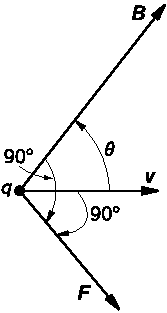
\includegraphics[width=0.5\linewidth]{fyz_fig061.pdf}
      \caption{Složka síly působící na pohybující se náboj závislá na rychlosti je kolmá na 
               \(\vec{v}\) a na směr \(\vec{B}\). Je úměrná složce \(\vec{v}\) kolmé na 
               \(\vec{B}\), tj. úměrná v \(\sin\vartheta\). O existenci magnetické síly se snadno 
                přesvědčíme, přiložíme-li tyčový magnet těsně k obrazovce. Vychýlení elektronového 
                paprsku svědčí o tom, že přítomnost magnetuje projevuje silou působící na 
                elektrony, která je kolmá na směr jejich pohybu, jak to bylo popsáno v kapitole 
                \ref{fyz:IchapXII}, odstavci \ref{fyz:IchapXIIsecIV}.
                \cite[s.~225]{Feynman02}}
      \label{fyz:fig061}
    \end{figure}
    
    Jednotka magnetického pole je zřejmě \(\text{newton}\cdot\text{sekunda}\) na \(\text{coulomb} 
    \cdot \text{metr}\). A stejnou jednotkou je i \(\text{volt}\cdot\text{sekunda}\) na metr 
    čtvereční. Nazývá se \emph{weber na metr čtvereční} nebo \emph{tesla}.

    \subsection{Elektrický proud, zachování náboje}
      \cite[s.~225]{Feynman02} Zamyslíme se nad tím, jak je možné chápat magnetické síly působící 
      na vodiče, jimiž tečou elektrické proudy. Musíme si ujasnit, co budeme chápat pod proudovou 
      hustotou. Elektrické proudy, to jsou elektrony nebo jiné náboje pohybující se takovým 
      způsobem, že v souhrnu vytváří tok v jistém směru. Hustotu toku náboje můžeme charakterizovat 
      vektorem, který určuje množství náboje procházejícího za jednotku času jednotkovou plochou 
      povrchovým elementem kolmým na směr toku (stejně jako v případě tepelného toku). Takovýto tok 
      nazýváme proudová hustota a označujeme jej vektorem \(\vec{j}\) Tento vektor směřuje podél 
      pohybu náboje. Zvolíme-li malou plošku \(\Delta S\) v daném místě látky, množství náboje 
      protékající touto ploškou za jednotku času můžeme vyjádřit ve tvaru
      \begin{equation}\label{eq_fyz:mag001}
        \vec{j}\cdot\vec{n}\Delta S,
      \end{equation} 
      kde \(\vec{n}\) je jednotkový vektor normály k ploše \(\Delta S\).
      
      Proudová hustota souvisí se střední rychlostí toku nábojů. Předpokládejme takové rozdělení 
      nábojů, které vede k usměrněnému pohybu se střední hodnotou rychlosti \(v\). Prochází-li 
      toto rozdělení povrchovým elementem \(\Delta S\), je náboj \(\Delta q\) procházející za čas 
      \(\Delta t\) povrchovým elementem roven náboji obsaženému v rovnoběžnostěnu se základnou 
      \(\Delta S\) a výškou \(v\Delta t\), jak to ukazuje obr. \ref{fyz:fig216}.
      \begin{figure}[ht!]
        \centering
        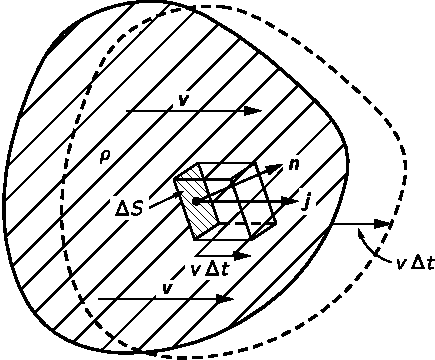
\includegraphics[width=0.7\linewidth]{fyz_fig216.pdf}
        \caption{Pohybuje-li se náboj rozložený s hustotou \(\varrho\) rychlostí \(v\), projde za 
        jednotku času plochou \(\Delta S\) náboj \(\varrho\vec{v}\cdot\vec{n}\Delta S\)}
        \label{fyz:fig216} 
      \end{figure}
      
      Objem tohoto rovnoběžnostěnu je součinem dvou faktorů, z nichž jeden je \(v\Delta t\) druhý 
      je průmět \(\Delta S\) do roviny kolmé na \(\vec{v}\). Násobíme-li tento objem hustotou 
      náboje \(\varrho\), dostaneme \(\Delta q\). Proto můžeme psát
      \begin{equation}\label{eq_fyz:mag002}
        \Delta q = \varrho\vec{v}\cdot\vec{n}\Delta S\Delta t.
      \end{equation}
      Náboj, který prošel za jednotku času, je pak roven \(\varrho\vec{v}\cdot\vec{n}\Delta S\), a 
      proto máme
      \begin{equation}\label{eq_fyz:mag003}
        \vec{j} = \varrho\vec{v}.
      \end{equation}
      
      Skládá-li se rozdělení nábojů z jednotlivých nábojů, např elektronů, z nichž každý má náboj 
      \(q\) a pohybují se střední rychlostí \(v\), můžeme proudovou hustotu vyjádřit ve tvaru
      \begin{equation}\label{eq_fyz:mag004}
        \vec{j} = Nq\vec{v}.
      \end{equation}
      
      Celkový náboj procházející za jednotku času nějakou plochou \(S\) se nazývá \emph{elektrický 
      proud} .Je roven integrálu normálové složky toku všemi elementy povrchu (obr. 
      \ref{fyz:fig217}):
      \begin{equation}\label{eq_fyz:mag005}
        I = \int\vec{j}\cdot\vec{n}\dd{S}.
      \end{equation}
    
      \begin{figure}[ht!]
        \centering
        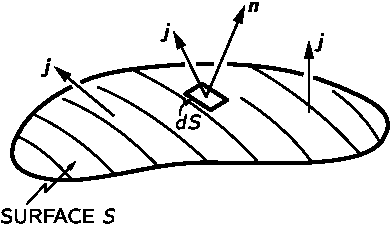
\includegraphics[width=0.5\linewidth]{fyz_fig217.pdf}
        \caption{Proud \(I\) procházející plochou \(S\) je roven \(\int\vec{j}\cdot\vec{n}\dd{S}\)}
        \label{fyz:fig217} 
      \end{figure}
      Proud vycházející z uzavřené plochy \(S\) představuje rychlost, s níž náboj opouští objem 
      \(V\) ohraničený plochou \(S\). Jeden ze základních fyzikálních zákonů hovoří o tom, že 
      elektrický náboj je nezničitelný, nikdy se neztrácí a nevzniká. Elektrické náboje se mohou 
      pohybovat z místa na místo, ale nikdy se neobjevují z ničeho nic. Říkáme, že náboj se 
      zachovává. Vytéká-li v konečném důsledku z uzavřené plochy proud, musí se odpovídajícím 
      způsobem zmenšovat množství náboje v objemu ohraničeném touto plochou (obr. 
      \ref{fyz:fig218}). Zákon zachování náboje proto lze vyjádřit ve tvaru
      \begin{equation}\label{fyz:eq_mag004} 
        \limitoint_{\mathclap{\substack{\text{libovolná}\\\text{uzavřená}\\\text{plocha}}}}
        \vec{j}\cdot\vec{n}\dd{S} = -\der{Q}{t}.
      \end{equation} 
      \begin{figure}[ht!]
        \centering
        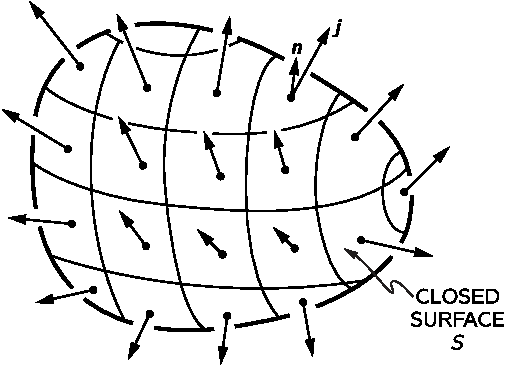
\includegraphics[width=0.5\linewidth]{fyz_fig218.pdf}
        \caption{Integrály \(\vec{j}\cdot\vec{n}\) přes uzavřenou plochu je roven rychlosti změny 
                 celkového náboje \(Q\) uvnitř této plochy.}
        \label{fyz:fig218} 
      \end{figure}
      Vnitřní náboj můžeme vyjádřit jako objemový integrál hustoty náboje
      \begin{equation}\label{fyz:eq_mag005} 
        Q_{\text{uvnitř}} = 
         \limitint_{\mathclap{\substack{V\\\text{uvnitř}\\\text{S}}}}\varrho\dd{V}.
      \end{equation}
      
      Použijeme-li vztah (\ref{fyz:eq_mag004}) pro malý objem \(\dd{V}\), integrál na levé straně 
      (\ref{fyz:eq_mag004}) je roven \(\nabla\cdot\vec{j}\Delta V\). Vnitřní náboj je 
      \(\varrho\Delta V\) a proto zákon zachování náboje lze napsat i ve tvaru
      \begin{equation}\label{fyz:eq_mag006}    %\ref{fyz:eq_mag006}
        \nabla\cdot\vec{j} = -\pder{\varrho}{t}
      \end{equation}
      (Opět \hyperlink{fyz:IIchapIIIsecIII}{Gaussova věta} z matematiky!)

    \subsection{Magnetická síla působící na proud}
      \cite[s.~227]{Feynman02} Nyní už jsme připraveni k tomu, abychom určili sílu, jež působí v 
      magnetickém poli na vodič, kterým teče proud. Proud se skládá z nabitých částic, které se 
      pohybují podél vodiče rychlostí \(v\). Na každý náboj působí příčná síla (obr. 
      \ref{fyz:fig219}).
      \begin{equation}\label{fyz:eq_mag007}
        \vec{F} = q\vec{v}\times\vec{B}
      \end{equation}
      \begin{figure}[ht!]
        \centering
        \begin{tabular}{cc}
          \subfloat[ ]{\label{fyz:fig219a}
            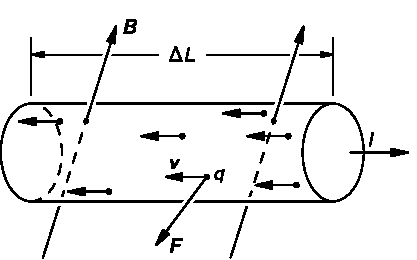
\includegraphics[width=0.45\linewidth]{fyz_fig219a.pdf}}              &
          \subfloat[ ]{\label{fyz:fig219b} 
            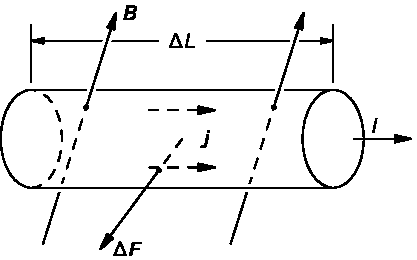
\includegraphics[width=0.45\linewidth]{fyz_fig219b.pdf}}
        \end{tabular}
        \caption{Magnetická síla působící na vodič, jímž protéká proud, je rovna součtu sil 
                 působících na jednotlivé pohybující se náboje}
        \label{fyz:fig219} 
      \end{figure}
      Je-li v objemové jednotce \(N\) takových nábojů, pak v malém objemu vodiče je jich \(N\Delta 
      V\). Celková magnetická síla \(\Delta F\) působící na objem \(\Delta V\) je součtem sil 
      působících na jednotlivé náboje, tj.
      \begin{equation}\label{fyz:eq_mag008}
        \Delta\vec{F} = (N\Delta V)(q\vec{v}\times\vec{B}).
      \end{equation}
      Jenže \(Nqv\) je právě \(\vec{j}\), a proto
      \begin{equation}\label{fyz:eq_mag009}
      \Delta\vec{F} = \vec{j}\times\vec{B}\Delta V.
      \end{equation}
      Jestliže vodičem, jehož plocha příčného řezu je rovna \(S\), teče proud rovnoměrně, můžeme 
      za objemový element zvolit válec se základnou \(S\) a délkou \(\Delta L\). Potom
      \begin{equation}\label{fyz:eq_mag010}
      \Delta\vec{F} = \vec{I}\times\vec{B}\Delta L.
      \end{equation}
      Síla působící na jednotkovou délku vodiče je rovna \(\vec{I}\times\vec{B}\).
      
      Tato rovnice vyjadřuje důležitý výsledek, který spočívá v tom, že magnetická síla působící 
      na vodič proto, že se v něm pohybují náboje, závisí jen na celkovém proudu, a ne na množství 
      náboje neseného každou z částic nebo dokonce na jeho znaménku! Magnetická síla, která v 
      blízkosti magnetu působí na vodič, se projeví vychýlením vodiče při zapnutí proudu tak, jak 
      to bylo popsáno v 1. kapitole (obr. 1.6)

    \subsection{Magnetické pole stacionárních proudů, Ampérův zákon}
      Viděli jsme, že na vodič v magnetickém poli vytvářeném např. magnetem působí síla. Podle 
      zákona akce a reakce bychom mohli očekávat, že bude existovat síla působící na zdroj 
      magnetického pole, tj. na magnet, když vodičem protéká proud\footnote{Později však uvidíme, 
      že takovýto předpoklad není obecně správný pro elektromagnetické síly!}. Takové síly opravdu 
      existují a můžeme se o nich přesvědčit pozorováním odklonu střelky kompasu v blízkosti 
      vodiče, jímž prochází elektrický proud. Dále víme, že mezi magnety existuje silové působení, 
      a proto můžeme usuzovat, že vodič sám vytváří magnetické pole, když jím teče proud. 
      Pohybující se náboje tedy \emph{vytvářejí} magnetické pole. Nyní se pokusme najít zákony, 
      jež určují, jaká pole se vytvoří. Otázka zní: Je-li dán proud, jaké bude magnetické pole jím 
      vytvořené? Odpověď na tuto otázku daly tři kritické experimenty a Ampérův důmyslný 
      teoretický důkaz. Přeskočíme tento zajímavý historický vývoj a pouze se zmíníme o tom, že 
      platnost Maxwellových rovnic byla dokázána velkým počtem experimentů. Maxwellovy rovnice 
      budou naším výchozím bodem. Zanedbáme-li v těchto rovnicích členy obsahující derivace podle 
      času, dostaneme rovnice magnetostatiky.
      \begin{align}
        \nabla\cdot\vec{B}     &= 0                            \label{fyz:eq_mag011} \\
        c^2\nabla\times\vec{B} &= \frac{\vec{j}}{\epsilon_0}.  \label{fyz:eq_mag012}
      \end{align}
      Tyto rovnice platí jen tehdy, jsou-li všechny hustoty elektrických nábojů konstantní a 
      všechny proudy stacionární, takže elektrická a magnetická pole se s časem nemění - obě pole 
      jsou \emph{stacionární}
      
      Je třeba poznamenat, že předpoklad statické magnetické situace není docela oprávněn, neboť 
      ke vzniku magnetického pole jsou potřebné proudy - a proudy vznikají pouze při pohybu nábojů. 
      Magnetostatika je proto pouze \emph{aproximací}. Souvisí se speciálním druhem dynamické 
      situace, kdy se pohybuje \emph{velký počet} nábojů a tento pohyb lze aproximovat 
      \emph{ustáleným} tokem náboje. Jen tehdy můžeme hovořit o proudové hustotě \(\vec{j}\), 
      která se v čase nemění. Kdybychom chtěli být přesnější, měli bychom tuto část nazývat 
      zkoumáním stacionárních proudů. Předpokládáme-li stacionárnost všech polí, můžeme v úplném 
      systému Maxwellových rovnic (\ref{fyz:eq266}) vynechat členy s \(\pder{\vec{E}}{t}\) a 
      \(\pder{\vec{B}}{t}\), a tak dostaneme již uvedenou dvojici rovnic (\ref{fyz:eq_mag011}) a 
      (\ref{fyz:eq_mag012}). Všimněte si, že divergence rotace libovolného vektoru je nevyhnutelně 
      nula, a proto rovnice (\ref{fyz:eq_mag012}) vyžaduje, aby \(\nabla\cdot\vec{j} = 0\). 
      Platí-li rovnice (\ref{fyz:eq_mag006}), bude to splněno pouze tehdy, když 
      \(\pder{\varrho}{t}\) rovno nule. To platí tehdy, když se \(\vec{E}\) s časem  nemění, takže 
      naše předpoklady jsou konzistentní.
      
      Podmínka \(\nabla\cdot\vec{j} = 0\) znamená, že můžeme uvažovat jen takové náboje, které se 
      pohybují po \emph{uzavřených dráhách}. Můžou např. téct ve vodičích tvořících uzavřené 
      smyčky, které nazýváme obvody. Obvody mohou, samozřejmě obsahovat generátory nebo baterie, 
      které udržují tok nábojů. Nesmí však obsahovat kondenzátory, které se nabíjejí nebo 
      vybíjejí. (Později, samozřejmě, rozšíříme teorii i na dynamická pole, ale nejdříve se budeme 
      zabývat jednodušším případem stacionárních proudů.)
      
      Nyní si všimneme rovnic (\ref{fyz:eq_mag011}) a (\ref{fyz:eq_mag012}) a zamyslíme se nad 
      tím, co znamenají. První rovnice říká, že divergence \(\vec{B}\) je rovna nule. Porovnáme-li 
      ji s analogickou rovnicí elektrostatiky, která říká, že \(\nabla\cdot\vec{E} = 
      \frac{\varrho}{\epsilon_0}\), zjistíme, že neexistuje magnetická analogie elektrického 
      náboje. \textbf{Neexistují magnetické náboje}, z nichž by mohly vycházet čáry \(\vec{B}\). 
      Budeme-li v našich úvahách používat pojem \emph{„indukční čáry“} vektorového pole 
      \(\vec{B}\), tyto nebudou nikde začínat a nikde končit. Odkud tedy pocházejí? Magnetická 
      pole se \emph{„objevují“} v \emph{přítomnosti} proudů; mají rotaci úměrnou proudové hustotě. 
      Kdekoliv jsou proudy, jsou tam i čáry magnetického pole vytvářející smyčky okolo proudů. 
      Protože čáry \(\vec{B}\) nezačínají a nekončí, často se uzavírají do sebe a vytvářejí 
      uzavřené smyčky. Mohou však existovat složité situace, v nichž čáry nejsou jednoduchými 
      uzavřenými smyčkami. Ale ať procházejí kudykoliv, nikdy nevycházejí z bodů. Magnetické 
      náboje nebyly nikdy objeveny, a proto \(\nabla\cdot\vec{B} = 0\). Platí to vždy - nejen pro 
      \emph{magnetostatiku}, ale i pro \emph{dynamická pole}.
      
      Souvislost mezi polem \(\vec{B}\) a proudy je vyjádřen rovnicí (\ref{fyz:eq_mag012}). Máme 
      novou situaci, zcela odlišnou od elektrostatiky, kde platilo \(\nabla\times\vec{E}=0\). 
      Takový vztah znamenal, že křivkový integrál z \(\vec{E}\) po libovolné uzavřené dráze je 
      roven nule:
      \begin{equation}\label{fyz:eq_mag013} 
        \limitoint_{\mathclap{\substack{\text{po smyčce}}}}\vec{E}\cdot\dd{\vec{s}} = 0.
      \end{equation} 
      Tento výsledek jsme získali ze \hyperlink{fyz:sec_002}{Stokesovy věty}, která říká, že 
      integrál po libovolné uzavřené dráze jakéhokoliv vektorového pole je roven plošnému 
      integrálu normálové složky rotace vektoru (integrál bereme po libovolné ploše, která má jako 
      svou hranici uzavřenou smyčku). Kdybychom tutéž větu použili v případě vektoru magnetického 
      pole, dostali bychom použitím symbolů z obr. \ref{fyz:fig220}.
      \begin{equation}\label{fyz:eq_mag014} 
      \limitoint_{\mathclap{\substack{\Gamma}}}\vec{B}\dd{\vec{s}} = \vec{E}\cdot\vec{n}\dd{S} = 0.
      \end{equation} 
      
      \begin{figure}[ht!]
        \centering
        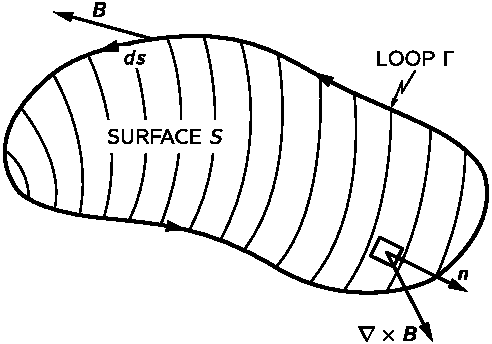
\includegraphics[width=0.5\linewidth]{fyz_fig220.pdf}
        \caption{Křivkový integrál tangenciální složky \(\vec{B}\) je roven plošnému integrálu 
                 normálové složky \(\nabla\times\vec{B}\).}
        \label{fyz:fig220} 
      \end{figure}

  \section{Elektrický proud. Zachování náboje}\label{fyz:IIchapXIIIsecII}
  \section{Magnetická síla působící na proud}\label{fyz:IIchapXIIIsecIII}
  \section{Magnetické pole stacionárních proudů. Ampérův zákon }\label{fyz:IIchapXIIIsecIV}
  \section{Magnetické pole přímého vodiče a solenoidu. Atomové 
  proudy}\label{fyz:IIchapXIIIsecV}
  \section{ Magnetická a elektrická pole v teorii relativity}\label{fyz:IIchapXIIIsecVI}
  \section{Transformace proudů a nábojů}\label{fyz:IIchapXIIIsecVII}
  \section{Superpozice. Pravidlo pravé ruky}\label{fyz:IIchapXIIIsecVIII}


    \begin{figure}[ht!] %\ref{fyz_fig683}
      \centering
      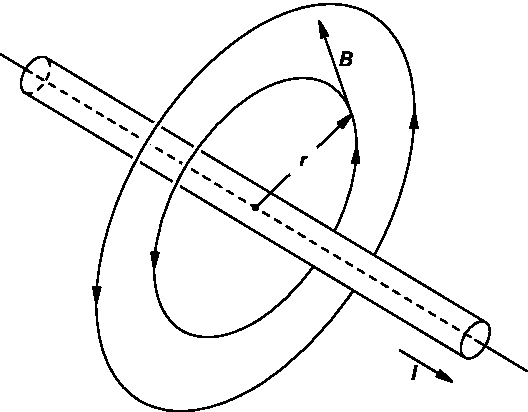
\includegraphics[width=0.7\linewidth]{fyz_fig683.pdf}
      \caption{
               (\cite[s.~707]{Feynman02})}
      \label{fyz_fig683}
    \end{figure}

    \begin{figure}[ht!] %\ref{fyz_fig684}
      \centering
      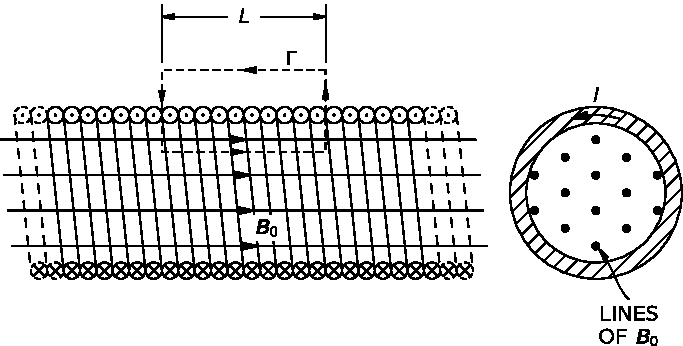
\includegraphics[width=0.7\linewidth]{fyz_fig684.pdf}
      \caption{
               (\cite[s.~707]{Feynman02})}
      \label{fyz_fig684}
    \end{figure}

    \begin{figure}[ht!] %\ref{fyz_fig685}
      \centering
      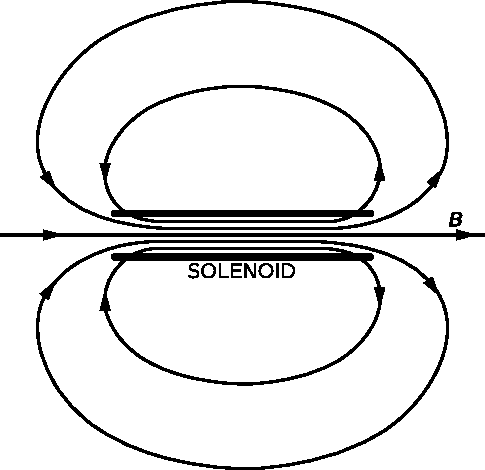
\includegraphics[width=0.7\linewidth]{fyz_fig685.pdf}
      \caption{
               (\cite[s.~707]{Feynman02})}
      \label{fyz_fig685}
    \end{figure}

    \begin{figure}[ht!] %\ref{fyz_fig686}
      \centering
      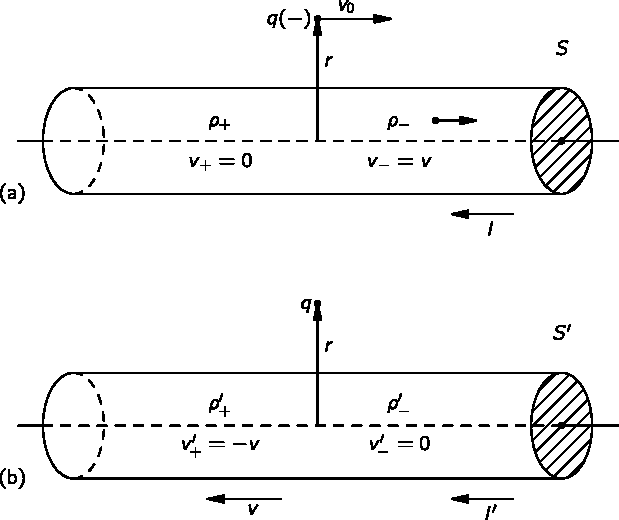
\includegraphics[width=0.7\linewidth]{fyz_fig686.pdf}
      \caption{
               (\cite[s.~707]{Feynman02})}
      \label{fyz_fig686}
    \end{figure}

    \begin{figure}[ht!] %\ref{fyz_fig687}
      \centering
      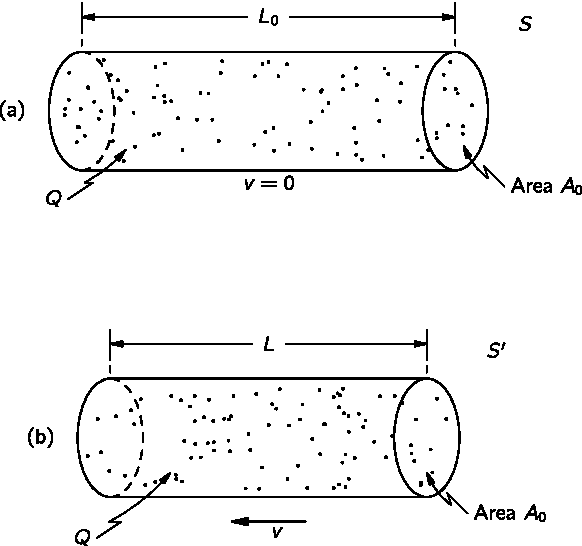
\includegraphics[width=0.7\linewidth]{fyz_fig687.pdf}
      \caption{
               (\cite[s.~707]{Feynman02})}
      \label{fyz_fig687}
    \end{figure}

    \begin{figure}[ht!] %\ref{fyz_fig688}
      \centering
      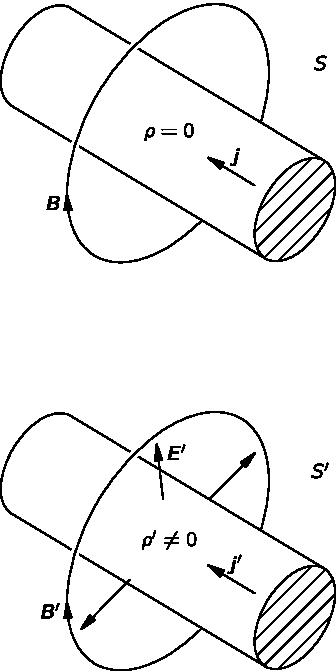
\includegraphics[width=0.7\linewidth]{fyz_fig688.pdf}
      \caption{
               (\cite[s.~707]{Feynman02})}
      \label{fyz_fig688}
    \end{figure}


} %tikzset
%~~~~~~~~~~~~~~~~~~~~~~~~~~~~~~~~~~~~~~~~~~~~~~~~~~~~~~~~~~~~~~~~~~~~~~~~~~~~~~~~~~~~~~~~~~~~~~~~~~
\printbibliography[title={Seznam literatury}, heading=subbibliography]
\addcontentsline{toc}{section}{Seznam literatury}